\section{Experiments}

To assess the efficacy of our method, we initially evaluate its ability to improve the token acceptance rate ($\alpha$) 
within an offline context. 
This provides us with a theoretical upper bound on the performance improvements achievable when the query distribution remains constant. 
Subsequently, we examine the approach's impact in an online environment, discovering that the acceptance rate improves even with a moderate amount of data while maintaining 
accuracy levels comparable to those in the offline scenario. 
Throughout our experiments, we employ two target models ($M_p)$: Vicuna-7B~\citep{vicuna2023} and FLAN-T5-XL (3B)~\citep{chung2022scaling}. Specifically for Vicuna-7B, we utilize LLaMA-160m~\citep{miao2023specinfer} as the draft model ($M_q$). For FLAN-T5-XL, we use T5-Small~\citep{raffel2020exploring} as the draft model. 
We evaluate performance across four diverse datasets: Text-to-SQL (Spider)~\citep{yu2018spider}, graduate school math (Gsm8k)~\citep{cobbe2021gsm8k}, Python code generation (Code-search-Python)~\citep{husain2019codesearchnet}, and financial question answering (Alpaca-finance)~\citep{alpaca-finance}. 
In all experiments, we set the number of proposed tokens to 5 for speculative decoding. For all online experiments, we fix the update interval \( I \) at 8. %

\subsection{Offline Evaluation}
\label{sec:offline-eval}
In this section, we assess the efficacy of employing knowledge distillation to train a small model specifically for speculation in an offline environment. 
In such a setting, the speculative $M_q$ model has unrestricted access to the dataset, and the query distribution remains stable. 
To emulate these offline conditions, we distill the $M_q$ using the training dataset for two epochs and subsequently evaluate its performance by measuring 
the average token acceptance rate ($\alpha$) on the test set.
As detailed in Section~\ref{sec:knowledge-distill}, we evaluated various sampling methods, namely teacher sampling, student sampling, and mix token-level sampling. 
Table~\ref{tab:apha} displays the token acceptance rate of the draft model for each method, using forward KL as the distance metric on the test dataset. 
For comparison, we also provide the acceptance rate for teacher-generated label fine-tuning and the original model.

For both the Vicuna-7B and FLAN-T5-XL models, the teacher sampling method outperforms others by achieving the highest acceptance rate. 
Furthermore, knowledge distillation has proven its efficacy in enhancing the draft model's approximation, resulting in a high token acceptance rate. Intriguingly, we also find that fine-tuning with teacher-generated labels yields impressive performance on the Vicuna-7B model. 
Lastly, we experimented with different distance measurements like reverse KL and JSD. %
Nevertheless, these measurements 
either paralleled or underperformed when compared to forward KL. 
Such empirical findings underscore that the optimal distance measurement or 
sampling method varies depending on the task and model, and we leave to future work to find the best combination. 


\begin{table}
\begin{small}
\caption{Token acceptance rates ($\alpha$) after two epochs. 
{\bf FT}: Finetuning on teacher-generated labels. 
{\bf TF, SF, MixF}: Teacher, student, and mix token sampling respectively, all with forward KL. %
}
\label{tab:apha}
\begin{center}
\begin{tabular}{lllllll}
\toprule
{\bf Model}                 & {\bf Task}         &{\bf Original} & {\bf FT} & {\bf TF }   & {\bf SF }    & {\bf MixF}\\
\midrule
\multirow{4}{*}{Vicuna-7B}  & Spider             &  0.28    & 0.74     & {\bf 0.76}         & 0.62         & 0.70  \\
                            & Gsm8k              &  0.58    & 0.74     & {\bf 0.75}         & 0.67         & 0.73  \\
                            & Code-search-Python &  0.38    & {\bf 0.65}     & {\bf 0.65}         & 0.51         & 0.61  \\
                            & Alpaca-finance     &  0.57    & {\bf 0.68}     & 0.67         & 0.63         & 0.65  \\
\hline
\multirow{4}{*}{FLAN T5-XL} & Spider  &    0.13  &  0.33  & \textbf{0.78}         &      0.67    &  0.70 \\
                            & Gsm8k              &  0.29    &  0.50    & \textbf{0.62}         &   0.51      & 0.55  \\
                            & Code-search-Python &  0.28   &  0.44   & \textbf{0.81}         &    0.67      & 0.78 \\              
                            & Alpaca-finance     &   0.39   &  0.56   & \textbf{0.63}         &    0.59      & 0.60  \\
\bottomrule
\end{tabular}
\end{center}
\end{small}
\vspace{-20pt}
\end{table}


\subsection{Online Evaluation}
\label{sec:eval:online_evaluation}
{\bf Online Learning.} First, we evaluate the effectiveness of our online algorithm by addressing two key questions: (1) Does the online algorithm increase the token acceptance rate? And is this enhancement comparable to the rates achieved in offline settings, which serve as an upper bound given their full access to data? (2) How quickly does the online algorithm increase the token acceptance rate, thereby indicating that the compact model has grasped the underlying distribution?

In our approach, we replicate the online serving process by iterating through the datasets, extracting prompts, and streaming generation requests. The system utilizes speculative decoding for each of these requests. Throughout this serving phase, we continually refine the speculative models, as detailed in Algorithm~\ref{algo:1}.
For our baseline, we envision a scenario where the serving system has the capability to collect data offline in order to distill an initial draft model. This model is subsequently deployed online to cater to future requests. This process is simulated by using 10\% of the dataset to distill the draft model, which remains static during online serving.
For evaluation metrics, we calculate token acceptance rates averaged over the most recent 50 requests. This demonstrates $M_q$'s efficacy on the most current data.

\begin{figure}[h]       
    \centering
    
\includegraphics[width=0.8\linewidth]{figures/legend_figure1.pdf}
    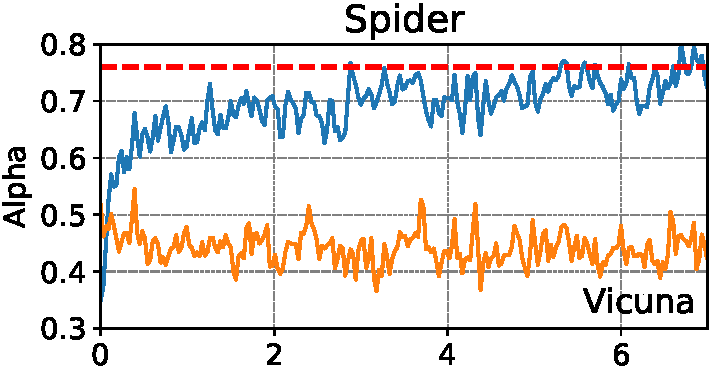
\includegraphics[width=0.256\linewidth]{figures/spider_vicuna.pdf}
    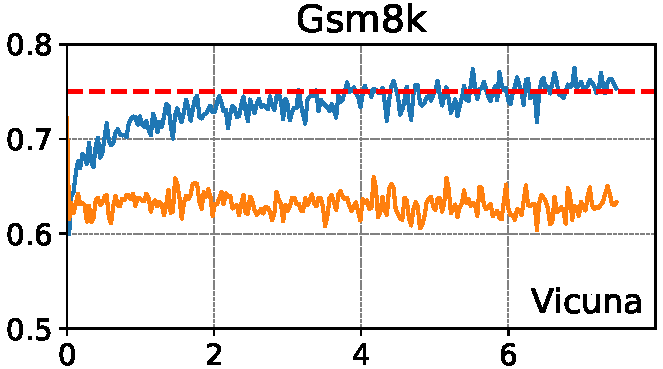
\includegraphics[width=0.242\linewidth]{figures/gsm8k_vicuna.pdf}
    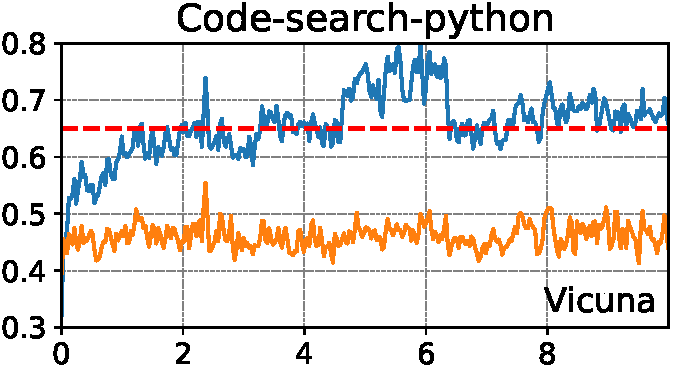
\includegraphics[width=0.24\linewidth]{figures/python_vicuna.pdf}
    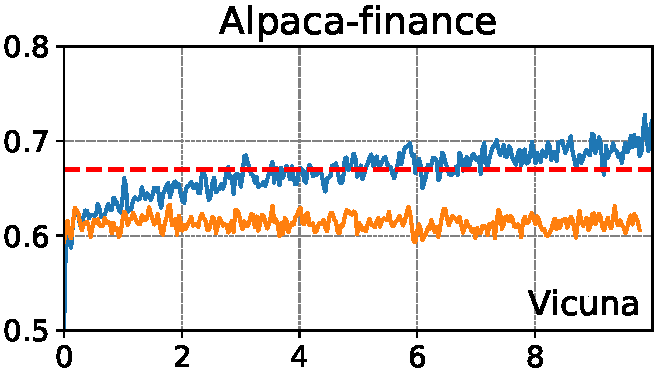
\includegraphics[width=0.24\linewidth]{figures/finance_vicuna.pdf}
    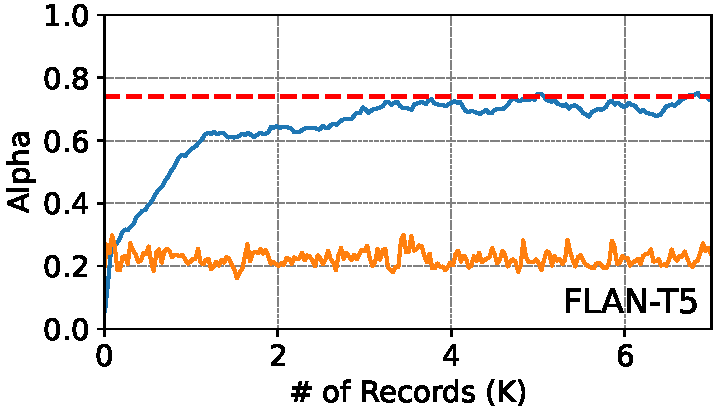
\includegraphics[width=0.259\linewidth]{figures/spider_flant5xl_to_t5small.pdf}
    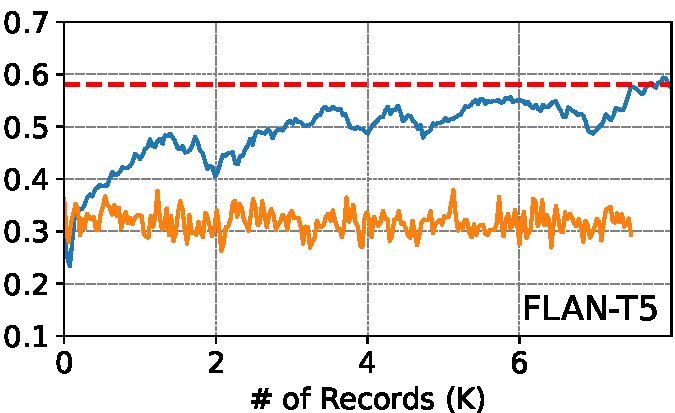
\includegraphics[width=0.24\linewidth]{figures/gsm8k_flant5xl_to_t5small.pdf}
    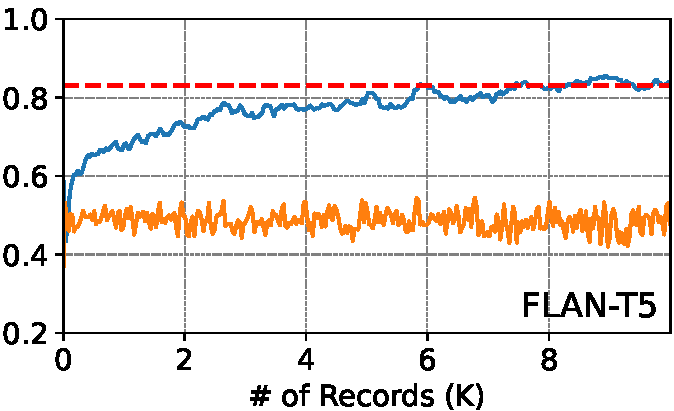
\includegraphics[width=0.24\linewidth]{figures/python_flant5xl_to_t5small.pdf}
    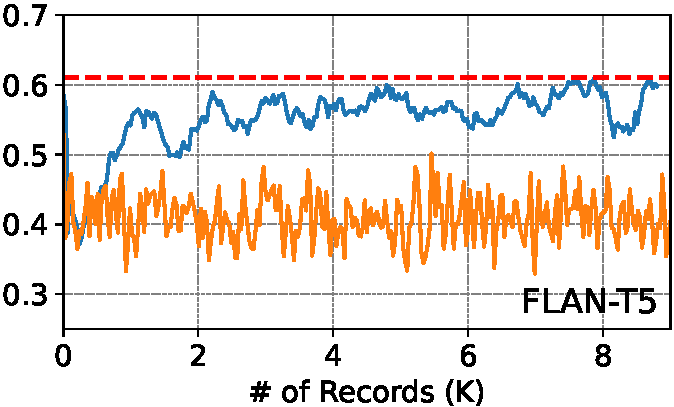
\includegraphics[width=0.24\linewidth]{figures/finance_flant5xl_to_t5small.pdf}
    \vspace{-15pt}
    \caption{Online acceptance rate ($\alpha$) across different datasets. The x-axis represents the number of records that \tool has processed. Alpha is averaged over the most recent 50 records.}
    \label{fig:alphas}
\end{figure}

\begin{figure}      
\vspace{-10pt}
    \centering
    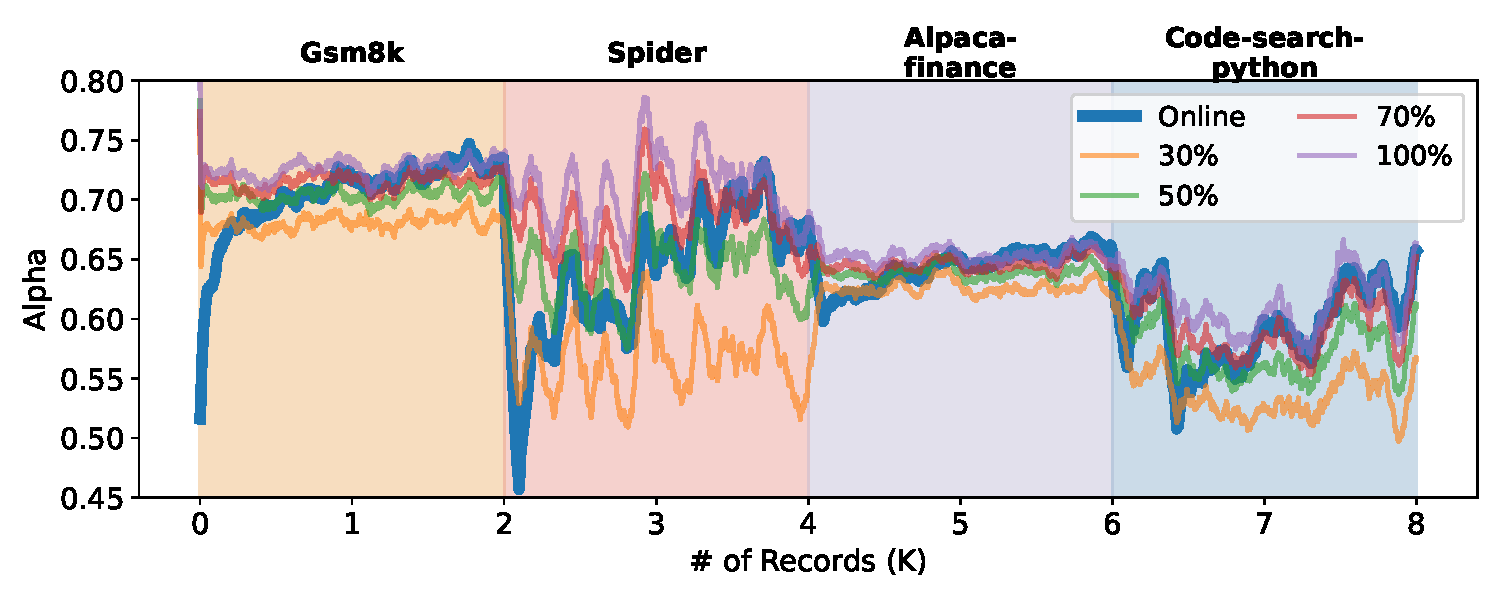
\includegraphics[width=0.75\linewidth]{figures/sharp.pdf}
    \vspace{-15pt}
    \caption{Distribution Shift: Alpha is averaged over the most recent 100 records.}
    \vspace{-15pt}
    \label{fig:dis-shift}
\end{figure}


As depicted in Figure 2, both for Vicuna-7B and FLAN-T5, in the beginning, \tool yields a lower token acceptance rate in comparison to the offline distilled model. Nevertheless, these acceptance rates rise swiftly as the draft model is exposed to more data. We also annotate the token acceptance rate from the offline setting to highlight the potential peak performance that the online serving system could reach. 
In all instances, the online context can achieve comparable results. In some scenarios, \tool even surpasses the token acceptance rate of the offline test alphas. This discrepancy can be attributed to the fact that offline test alphas are assessed on the entire test dataset, whereas the online alphas represent the moving average of the latest 50 requests. It's plausible that \tool performs optimally on specific data subsets, particularly if those subsets are more narrowly distributed than the complete dataset.

{\bf Distribution Shifts.} 
We evaluate \tool's ability to adapt to changes in data distribution. 
We detail the dataset preparation in Appendix~\ref{appendix:distribution-shift}. 
As illustrated in Figure~\ref{fig:dis-shift}, \tool's alpha value dips notably at distribution boundaries, especially around 2K, 4K, and 6K records. 
This is anticipated since the draft model initially struggles when faced with a new distribution. However, the alpha value rebounds quickly as \tool processes more data, highlighting its adaptability to shifting query distributions.

We also compared our results to those from a static setting. To ensure the draft model wasn't just memorizing data, we chose samples distinct from the online evaluation data. These samples correspond to 30\%, 50\%, 70\%, and 100\% of each dataset's online evaluation volume, at 0.6K, 1K, 1.4K, and 2K quantities respectively. As depicted in Figure~\ref{fig:dis-shift}, upon an initial shift in query distribution, \tool's performance aligns with or slightly trails the distillation with 30\% data. However, it quickly catches up, matching or even surpassing performances seen with 70\% to 100\% data access. This highlights \tool's ability to rival models fully exposed to the query distribution, even without intimate knowledge of the underlying query dynamics.


{\bf Real Workloads.} We evaluate \tool on real LMSYS-chat conversations (Appendix ~\ref{appendix:arena}) that span 4 months.
First, we categorize conversations based on the language and we focus on conversations among the top five languages, excluding English. For every chosen language, we use an independent LLaMA-160M to serve as our draft model. All draft models share the same Vicuna-7B as the target model. The token acceptance rate, averaged over the latest 100 requests, showed in Figure~\ref{fig:arena}, reveals that \tool's enhances rates by 0.1 to 0.2, even with under 2K data points. Notably, Japanese was the easiest while Portuguese was the toughest.
We also clustered English conversations by topics using the fine-tuned distilled Bert model~\citep{distill-bert-topic}, focusing on the top five. For topics with over 5K conversations, we sampled evenly to keep it within 5K. Figure~\ref{fig:arena} shows acceptance rates above 0.6 across topics, with Social and Computer discussions peaking near 0.8.
\begin{figure}
    \vspace{-10pt}
    \centering
    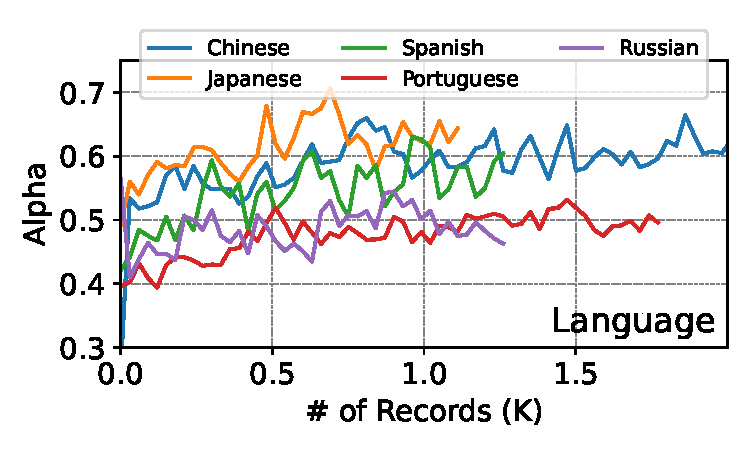
\includegraphics[width=0.4\linewidth]{figures/arena_language.pdf}
    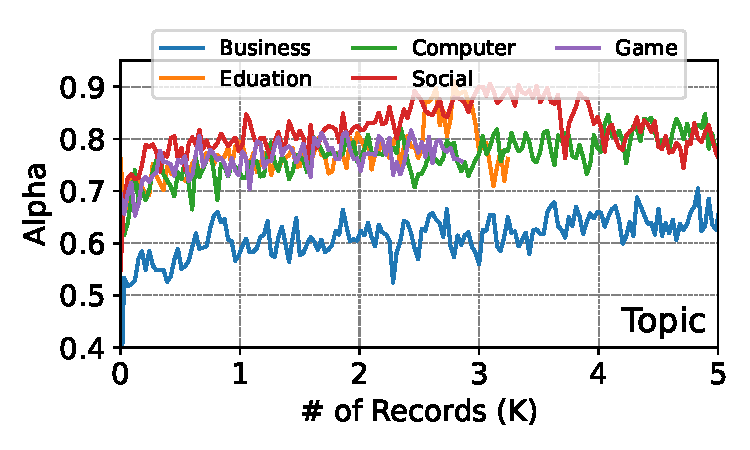
\includegraphics[width=0.4\linewidth]{figures/arena_class.pdf}
    \vspace{-10pt}
    \caption{Chatbot Arena Conversations clustered by language and topic.}
    \label{fig:arena}
\end{figure}

\begin{figure} 
    \vspace{-10pt}
    \centering
    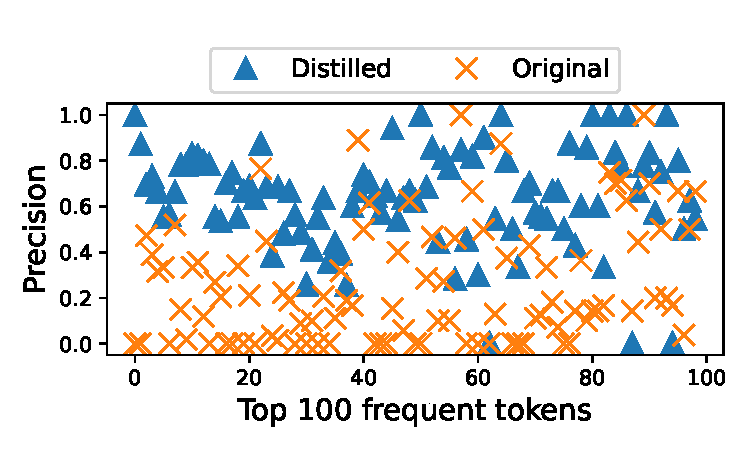
\includegraphics[width=0.4\linewidth]{figures/precision.pdf}
    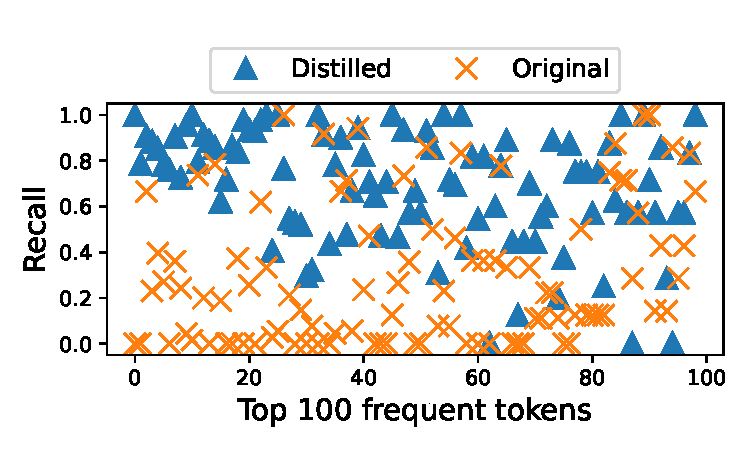
\includegraphics[width=0.4\linewidth]{figures/recall.pdf}
    \vspace{-10pt}
    \caption{Precision and recall of high-frequency tokens. The x-axis shows the rating of the tokens based on their occurrence in the generated answers. For instance, token 1 appears most frequently in answers. Precision = \#  of times token $i$ is accepted by the target model / \# of times token $i$ is proposed by the draft model. Recall = \# of times token $i$ is accepted by the target model / \# of times token $i$ appears in the final answer.}
    \label{fig:freq-acc}
    \vspace{-10pt}
\end{figure}


\subsection{Qualitative Analysis}
In this section, we conduct a comprehensive analysis to understand how our method enhances the token acceptance rate, and which tokens the draft model acquires across varying query distributions.

{\bf High-frequency tokens precision and recall.} In our experiment using the Spider dataset, Vicuna-7M is the target model and LLaMA-160M the draft. 
We identify the top 100 tokens most frequently generated by the target model, which account for 72.2\% of all appearances, 
following a power-law distribution. Figure~\ref{fig:freq-acc} shows a marked improvement in both accuracy and recall
of these tokens after distillation on the test dataset in an offline evaluation. 



\begin{table}[h!]
\vspace{-10pt}
\caption{Top 15 tokens with the most recall/precision improvement across datasets. We ignore \_ before tokens, which represents space in the LLaMA tokenizer.}
\label{tab:tokens}
\begin{center}
\begin{footnotesize}
\begin{tabular}{p{1.5cm}|p{2.4cm}|p{2.4cm}|p{2.4cm}|p{2.4cm}}
\toprule
{\bf Dataset} & {\bf Spider} & {\bf Gsm8k} & {\bf Alpaca-Finance} & {\bf Code-Python} \\
\midrule
{\bf Tokens with the greatest precision increase}
&
AV, SELECT, first, ⟨EOS⟩, template, SUM, G, COUNT, \textbackslash n, city, WHERE, ';, (, IST, id
&
⟨EOS⟩, \textgreater\textgreater, +, To, \textless\textless, this, =, \%, know, are, We, calculate, be, The, have
&
1, Here, (, :, provide, depends, However, goals, amount, 3, there, The, \textbackslash n, personal, will
&
''', (, Here, python, ', how, doc, snippet, import, based, \{, Python, This, :, you \\
\hline
{\bf Tokens with the greatest recall increase}
&
SELECT, *, FROM, (, IST, *), \textbackslash n, COUNT, G, first, WHERE, ⟨EOS⟩, IN, ;, MAX, ';
&
start, \textgreater\textgreater, \textless\textless, +, find, how, we, =, fore, To, so, \textbackslash, ⟨EOS⟩, then, let
&
general, 1, several, This, depends, Here, provide, However, goals, over, (, If, amount, it, can
&
Here, This, snippet, ''', ', how, python, (, takes, Python, you, doc, an, import, def \\
\bottomrule
\end{tabular}
\end{footnotesize}
\end{center}
\vspace{-10pt}
\end{table}

{\bf Tokens learned across different datasets}
In our study, we analyze the top 10 tokens with the most pronounced accuracy and recall improvements across various datasets, focusing on the 100 most frequent tokens to 
understand the draft model's learning trends. As detailed in Table~\ref{tab:tokens}, the improved tokens align well with the underlying data distribution. 
For example, in the Spider dataset, which frequently generates SQL statements, tokens like SELECT and WHERE have notably higher acceptance rates post-distillation. 
Similarly, in the Graduate Math dataset (Gsm8k), tokens such as \textless\textless, \textgreater\textgreater, =, and + stand out. 
These patterns highlight the draft model's ability to adapt and predict tokens consistent with the data distribution.













